本章主要用于测试该模版。

\subsection{结构}
图\ref{FPGA结构}为FPGA基本单元结构图。
\begin{figure}[H] % H为当前位置,!htb为忽略美学标准,htbp为浮动图形
    \centering
    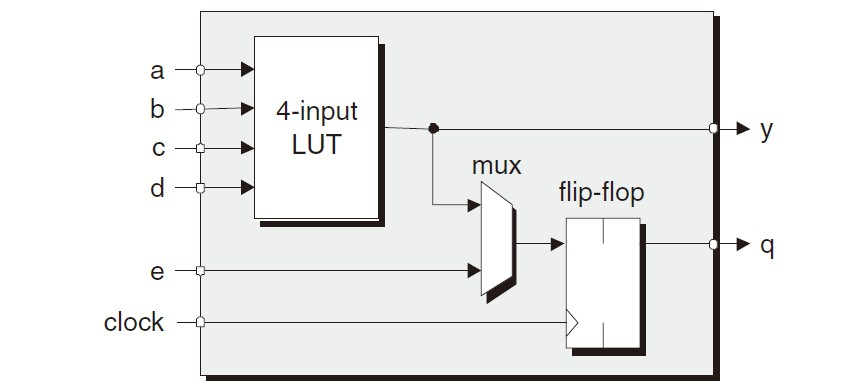
\includegraphics{img/FPGA.jpg}
    \caption{Slice of FPGA} %最终文档中希望显示的图片标题
    \label{FPGA结构} %用于文内引用的标签
\end{figure}

FPGA的基本单元是Slice,主要包括LUT、MUX及触发器,其中每个Slice的大小和FPGA型号有关。

\subsection{数学}
这里有一个数学公式
\begin{equation}
    \int_1^2 x dx = \frac{3}{2} 
\end{equation}

\subsubsection{数学公式说明}
这是一个简单的积分.

\subsection{代码}
推荐的verilog代码风格如下所示,但目前空格对齐的方式还没完全理解清楚。
\lstset{language=verilog}
\begin{lstlisting}
module keyboard(
    input           clk,
    input           rst_n,
    input  [3 : 0]  col,
    output [3 : 0]  key_pulse
);

reg  [11 : 0] treg0; // tmp reg
reg  [11 : 0] treg1; // tmp reg
reg  [11 : 0] treg2; // tmp reg
reg  [11 : 0] treg3; // tmp reg
wire [11 : 0] treg0_nxt = treg0 + 1'b1; // tmp reg next val
wire [11 : 0] treg1_nxt = treg1 + 1'b1; // tmp reg next val
wire [11 : 0] treg2_nxt = treg2 + 1'b1; // tmp reg next val
wire [11 : 0] treg3_nxt = treg3 + 1'b1; // tmp reg next val

// when tregx = 12'hffe and tregx_nxt = 12'hfff
// key_pulse will be 1
// then, tregx will be 12'hfff
// when tregx == 12'hfff, it will keep until keyboard not pushed
always @ (posedge clk or negedge rst_n) begin
    if (~rst_n) begin
        treg0 <= 12'b0;
        treg1 <= 12'b0;
        treg2 <= 12'b0;
        treg3 <= 12'b0;
    end
    else begin
        if (col[0]) begin 
            if (treg0 != 12'hfff) 
                treg0 <= treg0_nxt;
        end
        else begin
            treg0 <= 12'b0;
        end

        if (col[1]) begin
            if (treg1 != 12'hfff) 
                treg1 <= treg1_nxt;
        end
        else begin   
            treg1 <= 12'b0;
        end

        if (col[2]) begin
            if (treg2 != 12'hfff)
                treg2 <= treg2_nxt;
        end
        else begin
            treg2 <= 12'b0;
        end

        if (col[3]) begin
            if (treg3 != 12'hfff) 
                treg3 <= treg3_nxt;
        end
        else begin        
            treg3 <= 12'b0;
        end
    end
end

assign key_pulse[3] = (treg3 != 12'hfff) & (treg3_nxt == 12'hfff); 
assign key_pulse[2] = (treg2 != 12'hfff) & (treg2_nxt == 12'hfff);
assign key_pulse[1] = (treg1 != 12'hfff) & (treg1_nxt == 12'hfff);
assign key_pulse[0] = (treg0 != 12'hfff) & (treg0_nxt == 12'hfff);

endmodule
\end{lstlisting}